
\section{The Euler equation of turbomachinery}

In the following sections, we compute the torque and power transferred
by a turbomachine rotor to the flow.

\subsection{Torque}

The moment of momentum of an infinitely small parcel of fluid is
$\xyzV \times \dens \velV$; its rate of change is equal to the
integrated moment of the stress exerted on its boundary:
\begin{align*}
  \ddtM{} \int_\vol \xyzV \times \dens \velV =  \int_\vol \dens \xyzV \times \gravV~dV +
  \oint_{\srf} \xyzV \times \left(\stressT \cdot \nrmV \right)~dS
\end{align*}
Application of the transport theorem gives us 
\begin{equation}
  \int_\vol \ddt{} \left(\xyzV \times \dens \velV\right) ~dV +
  \oint_{\srf} \left(\xyzV \times \dens \velV\right) \cdot \left(\velV
    \cdot \nrmV\right)~dV = %\int_\vol \dens \xyzV \times \gravV~dV +
  \oint_{\srf} \xyzV \times \left(\stressT \cdot \nrmV \right)~dS
  \label{eq:momentOfMomentum}
\end{equation}
where $\stressT$ includes both pressure and shear stress
contributions.

\begin{figure}[!h]
  \begin{subfigure}{\textwidth}
    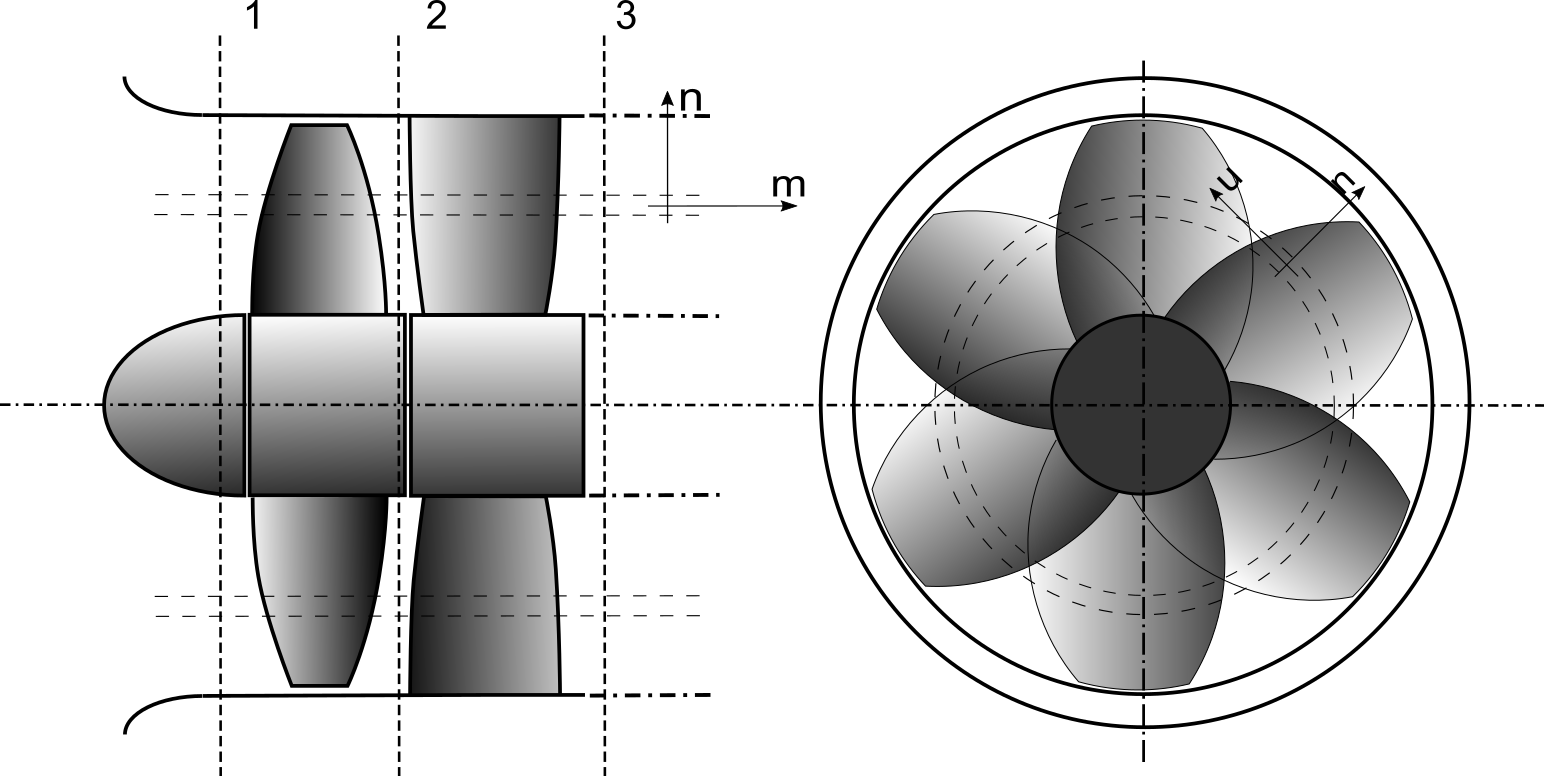
\includegraphics[width=\textwidth]{principles/ventilator_streamSurface.png}
    \caption{Axial ventilator - purely axial flow}
  \end{subfigure}
  \begin{subfigure}{\textwidth}
    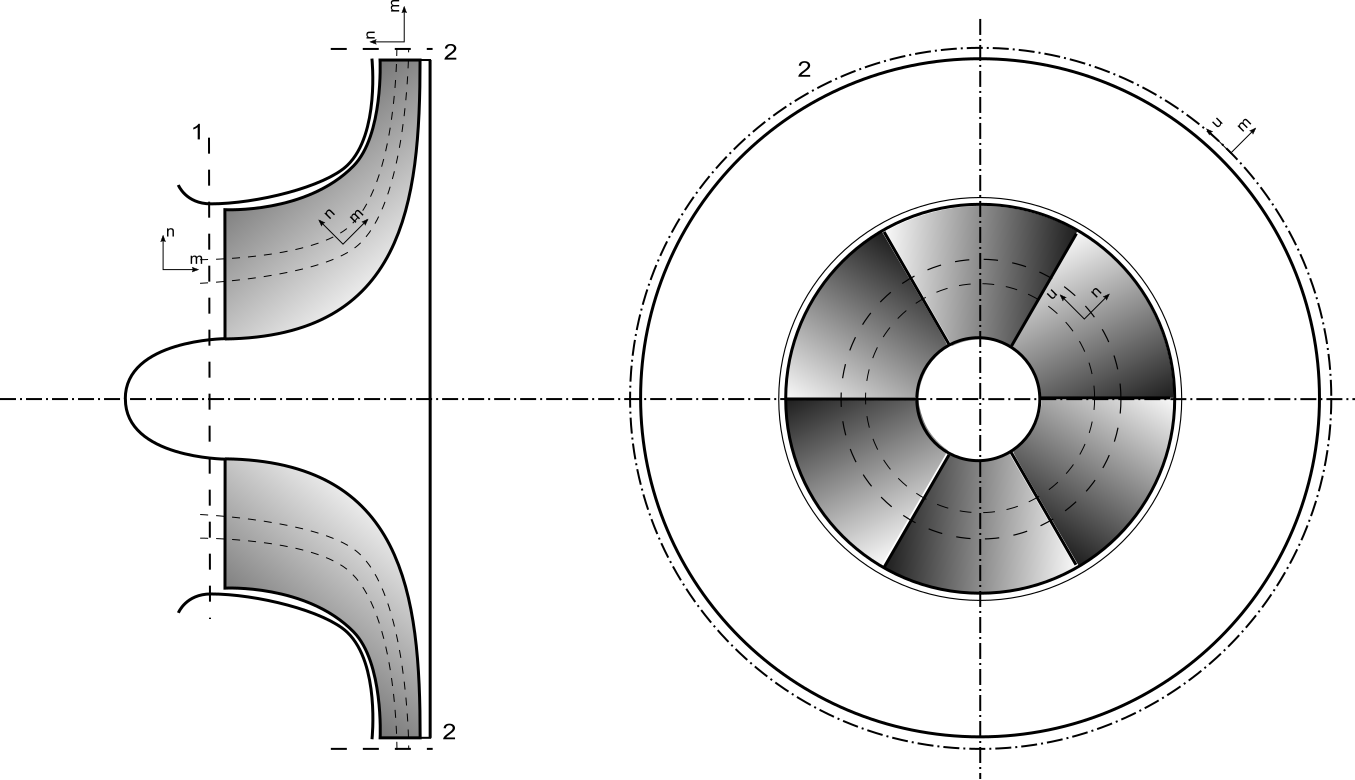
\includegraphics[width=\textwidth]{principles/centrifugalCompressor.png}
    \caption{Centrifugal compressor - axi-radial flow}
  \end{subfigure}
  \caption{Definition of global and streamsurface control volumes;
    local definition of meridional (m), normal(n) and circumferential
    (u) axes.}
  \label{fig:turbomachineControlVolumes}
\end{figure}
We can now use this equation to determine the torque applied to the
rotation axis of a turbomachine. Denoting the distance to the axis as
$\rad$, we find the following equation
\begin{equation}
  \int_\vol \ddt{} \dens \rad \vel_u ~dV + \oint_{\srf} \dens \rad \vel_u ~
  \left(\velV \cdot \nrmV\right)~dV = \int_\vol \dens \rad \grav_u~dV +
  \oint_{\srf} \rad \stress_{un} ~dS
  \label{eq:momentOfMomentumAxis}
\end{equation}
with $\stress_{un} = - p \nrm_u + \shearStress_{un}$.

We now apply this to a control volume delimited by the solid parts of
the rotor, namely the hub $H$, shroud $S$ and the blades $B_i$ on the
one hand, and two axisymmetric surfaces and at the in- (1) resp. the
outlet (2) as shown in figure
\ref{fig:turbomachineControlVolumes}. The latter two surfaces are
chosen at a sufficient distance from the blades. 

Assuming that that steady state is attained, the average torque is
found by integrating over the period of rotation $T = 2 \pi / \rot$.
\begin{itemize}
\item due to periodicity in time, the time derivative volume integral
  drops out;
\item due to symmetry, the integrated torque of gravity is zero;
\item there is no mass transport across the blades $\mathcal B_i$. The
  surface integral of the stress moment then provides us with the time
  average of the blade torque.
\item similarly there is no mass transport across the hub or
  shroud. Due to the axisymmetry\footnote{We make abstraction from
    some highly optimized turbomachines in which hub or shroud are no
    longer axisymmetric.} $\nrm_u=0$, and therefore the pressure
  exerts no moment, only viscous stresses do;
\item also the in- and outlet surfaces are axisymmetric, and
  therefore, there is no contribution of the pressure. Since the
  surfaces are chosen sufficiently far from the blades, no significant
  gradients are expected and hence $\shearStress_{nu} \approx
  0$. Therefore only the transport terms remain.
\end{itemize}
The torque on the rotor is given by the integral of the moment of the
stress on its rotating solid surfaces, comprised by the blades, the
hub and potentially the shroud. Assuming the shroud is attached to the
blades
\begin{align*}
  \torque = 
  \int_{H} \rad \shearStressT \cdot \nrmV dS + 
  \sum_i \int_{B_i} \rad \stressT \cdot \nrmV dS + 
  \int_{S} \rad \shearStressT \cdot \nrmV dS
\end{align*}
Therefore we find that the torque on the rotor is equal to the change
of moment of momentum of the flow from the inlet to the outlet
surface:
\begin{equation}
  \torque =
  \int_{2} \dens \rad \vel_u ~ \left(\velV \cdot \nrmV\right)~dV  - 
  \int_{1} \dens \rad \vel_u ~ \left(\velV \cdot \nrmV\right)~dV
  \label{eq:eulerMoment}
\end{equation}
Denoting the mass flow as $\mFlow$, we finally find
\begin{equation}
 \torque = \mFlow \left(
   \overline{\rad_2 \vel_{u2}} - 
   \overline{\rad_1 \vel_{u1}}\right) 
 \label{eq:eulerMoment2}
\end{equation}
where the $\overline{\rad \vel_u}$ denotes the mass flow average of
the moment of momentum.  If the shroud is not attached to the rotor,
its friction moment does not contribute to the torque exerted by the
rotor. However, it intervenes in the moment of momentum balance and
therefore the equation for the torque needs to be changed to:
\begin{equation}
  \torque = 
  \int_{2} \dens \rad \vel_u ~ \left(\velV \cdot \nrmV\right)~dV - 
  \int_{1} \dens \rad \vel_u ~ \left(\velV \cdot \nrmV\right)~dV 
  - \int_{S} \rad \shearStressT \cdot \nrmV dS  
  \label{eq:eulerMoment3}
\end{equation}

% \subsection{Torque seen in the relative frame}

% \todo{integration of $\xyzV \times $ momentum balance to show lift and
%   coriolis moment}

\subsection{Euler equation of turbomachinery}

The time-averaged power passing through the
machine rotating at angular velocity $\rot$ is then given by
\begin{align*}
  \power = \torque \omega = 
  \omega \mFlow \left(
    \overline {\rad_2 \vel_{u2}} - 
    \overline {\rad_1 \vel_{u1}}
  \right) = 
  \mFlow \left(
    \overline{\fVel_2 \vel_{u2}} - 
    \overline{\fVel_1 \vel_{u1}}\right)
\end{align*}
Conservation of total enthalpy then results in
\begin{equation}
  \mFlow (\overline \tEnth_2 - \overline \tEnth_1) = 
  \mFlow \left(
    \overline{\fVel_2 \vel_{u2}} - 
    \overline{\fVel_1 \vel_{u1}}
  \right)
  \label{eq:eulerPower}
\end{equation}
Equation \ref{eq:eulerPower} is the \emph{Euler equation of
  turbomachinery}.

We should note again that in case not all solid surfaces are attached
to the rotor, the moment $\torque$ in equation \ref{eq:eulerMoment} is
the combined moment on the rotor and the stator. The product of the
moment with the rotational speed in \ref{eq:eulerPower} then does not
(exactly) correspond to the power, as the rotor torque needs to be
corrected for the moment exerted by the shroud.

With some additional hypotheses, equations \ref{eq:eulerMoment} and
\ref{eq:eulerPower} can be used to analyse the variation of
torque and power contributions along the blade height. Therefore, we
assume flow evolves on axisymmetric surfaces. We then define an
axisymmetric control volume delimited by in- and outlet surfaces 1 and
2; two infinitesimally close stream surfaces $S_1$ and $S_2$ and
finally the part of the blade in between these two surfaces as shown
in figure \ref{fig:turbomachineControlVolumes}. There is supposedly no
flow across the surfaces $S_1$ and $S_2$, and due to their axisymmetry
$\nrm_u = 0$; therefore only shear stress contributions remain. These
contributions can again be considered small with respect to the moment
generated by the pressure on the blade; moreover, when such control
volumes are combined, the contributions on the common stream surfaces
drop out. The energy balance on this control volume then results in
\begin{equation}
  \begin{split}
  d \mFlow (\tEnth_2 - \tEnth_1) 
  &= d \mFlow \left(
    {u_2 \vel_{u2}} - 
    {u_1 \vel_{u1}}\right)  - (\int_{S1} u \shearStress_{un} dS 
  - \int_{S2} u \shearStress_{un} dS) \\
  &\approx d \mFlow \left(
    {u_2 \vel_{u2}} - 
    {u_1 \vel_{u1}}\right) 
  \end{split}
  \label{eq:eulerInfinitesimal}
\end{equation}
Finally, we should note that the conservation equation for moment of
momentum, nor the Euler equation for turbomachinery are fundamental
equations. As demonstrated above, they are consequences of the
Navier-Stokes equations, which can be found by integrating the moment
and energy equation on the appropriate control volume.

\subsection{Reaction rate}

The total enthalpy change across the rotor can be split up in on the
the static enthalpy change $\Delta h$ and the change in kinetic
energy. Going back to the Euler equation, the latter can be rewritten as
\begin{align*}
  \mFlow \left(
    \Delta \overline \enth + 
    \Delta \frac{\overline \aVel^2}{2}\right)
  &= \mFlow \Delta \overline{\fVel \aVel_{u}} = \mFlow \left(
    \frac{\Delta \overline \aVel^2}{2} + 
    \frac{\Delta \overline \rVel^2}{2} - 
    \frac{\Delta \overline \fVel^2}{2}\right)
\end{align*}
such that the static enthalpy rise is provided by the diffusion of the
relative velocity in the passage on the one hand and the centrifugal
pressure gradient on the other:
\begin{equation}
  \Delta \overline \enth = 
    \frac{\Delta \overline \rVel^2}{2} - 
    \frac{\Delta \overline \fVel^2}{2}
\end{equation}
In the absence of losses, the infinitesimal static enthalpy change is
proportional to the change in pressure since
\begin{align*}
  \temp d \entr = d\enth + \frac{d\pres}{\rho}
\end{align*}
The ratio of the static to the total enthalpy rise is called the
\emph{degree of reaction} \reaction, which is an important design
parameter. For driven machines (pumps, compressors), the higher it is,
the lower the kinetic energy that needs conversion by diffusion in
downstream stators, which is typically a process with high losses. For
turbines, a low degree of reaction requires a high acceleration in the
upstream stator in order to enable sufficient energy extraction in the
rotor. In multistage machines, and in particular compressors, one may
target an average degree of reaction of about 1/2, since then the
pressure gradients are evenly distributed over rotors and stators. 

\subsection{Velocity triangles}

We can define in any passage the average flow velocity $\aVelV$ over
the (axisymmetric) throughflow section between two stream surfaces, as
illustrated in figure \ref{fig:turbomachineControlVolumes}. In the
rotating parts, we also define the velocity $\rVelV$ relative to the
rotor. From section \ref{sec:principles:navierStokesRelative}, we know they
differ by the local rotor velocity $\fVelV$:
\begin{align*}
  \aVelV = \rVelV + \fVelV
\end{align*}
This relation is usually represented by the \emph{velocity} triangle,
illustrated in figure \ref{fig:velocityTriangle}. The triangle
decomposes the (stream-surface aligned) absolute and relative
velocities in two components. The \emph{meridional} component of both
absolute $\aVel_m$ and relative velocity $\rVel_m$ are the same, and
correspond to the volumetric flow rate following
\begin{align*}
  \vFlow_t = \aVel_m S = \aVel_m ~ 2 \pi R ~ h ~ (1-b)
\end{align*}
In this relation, $S$ is the throughflow surface, computed from
\begin{itemize}
\item the local radius;
\item the height $h$ of the flow passage of the control volume;
\item the blockage factor $b = 0.05 \ldots 0.1$ in case blades are
  present.
\end{itemize}
As found from the Euler equation, the energy transfer transferred to
the flow is determined by the \emph{tangential} components $\aVel_u$
and $\rVel_u$ of resp. the absolute and relative velocities. A useful
relation is then
\begin{align}
  \rVel^2 
  = \rVel_m^2 + \rVel_u^2 
  = \aVel_m^2 + \left(\aVel_u - \fVel\right)^2 
  \Rightarrow \fVel \aVel_u = \frac{\aVel^2}{2} - \frac{\rVel^2}{2} + \frac{\fVel^2}{2}
\end{align}
Within this course, the absolute and relative flow angles $\alpha$ and
$\beta$ are defined with respect to the meridional direction:
\begin{align*}
  \alpha &= \arctan \left(\frac{\aVel_u}{\aVel_m} \right) &
  \beta &= \arctan \left(\frac{\rVel_u}{\aVel_m} \right)
\end{align*}
Therefore the angles are defined as positive when the corresponding
velocity has the same tangential direction as the frame velocity
$\fVelV$.
\begin{figure}[!h]
  \centering{\tikzsetnextfilename{velocityTriangle}
\begin{tikzpicture}
  
  \coordinate(B) at (-4,0);
  \coordinate(A) at (8,0);
  \coordinate(C) at (0,4);
  \coordinate(D) at (0,0);
  
  % \node at (A) [circle,fill,inner sep=1.5pt]{};
  % \node at (B) [circle,fill,inner sep=1.5pt]{};
  % \node at (C) [circle,fill,inner sep=1.5pt]{};
  % \node at (D) [circle,fill,inner sep=1.5pt]{};
  
  \coordinate(Bp) at (-4,-1);
  \coordinate(Ap) at (8,-1);
  \coordinate(Dp) at (0,-1);
  
   \draw[->,>=latex,line width=1.5pt,color=red] 
  (C) -- (B) node [midway,sloped,above,color=red]{$\rVelV$};
  
  \draw[->,>=latex,line width=1.5pt] 
  (C) -- (D) node [midway,left,color=red]{$\rVel_m$};
  
  \draw pic["$\beta$", 
  draw=red,color=red, <-,>=latex, line width=1pt, angle eccentricity=1.3, angle radius=1cm]
  {angle=B--C--D} {};
  
  \draw[->,>=latex,line width=1.5pt,color=blue] 
  (C) -- (A) node [midway,sloped,above,color=blue]{$\aVelV$};
  
  \draw[->,>=latex,line width=1.5pt]
  (C) -- (D) node [midway,right,color=blue]{$\aVel_m$};
  
  \draw pic["$\alpha$", draw=blue,->,>=latex, line width=1pt, angle eccentricity=1.3, angle radius=1cm,color=blue]
  {angle=D--C--A} {};


  \draw[->,>=latex,line width=1.5pt] (B) --(A) node [midway,sloped,above]{$\fVelV$};;
  \draw[|->|,>=latex,color=red] (Dp) --(Bp) node[midway,sloped,above,color=red]{$\rVel_u$};
  \draw[|->|,>=latex,color=blue] (Dp) --(Ap) node[midway,sloped,above,color=blue]{$\aVel_u$};

  \draw[dashed] (A) -- (Ap);
  \draw[dashed] (B) -- (Bp);
  \draw[dashed] (D) -- (Dp);
  
\end{tikzpicture}
}
  \caption{Velocity triangle: absolute $\aVelV$, relative $\rVelV$ and
    frame velocity $\fVelV$; absolute $\alpha$ and relative flow angle
    $\beta$; meridional $\aVel_m,\rVel_m$ and tangential components
    $\aVel_u,\rVel_u$.}
  \label{fig:velocityTriangle}
\end{figure}

%%% Local Variables: 
%%% mode: latex
%%% TeX-master: t
%%% End: 
